
\section{I - Introduction}
\begin{frame}{I - Introduction}
	\begin{block}{Présentation du modèle du perceptron}
		C'est  en 1943, que McCulloh et Pitts introduisent le modèle du perceptron.  \\
		Ce modèle est basé sur le fonctionnement du neurone humain.
	\end{block}
	\begin{figure}
		\centering
		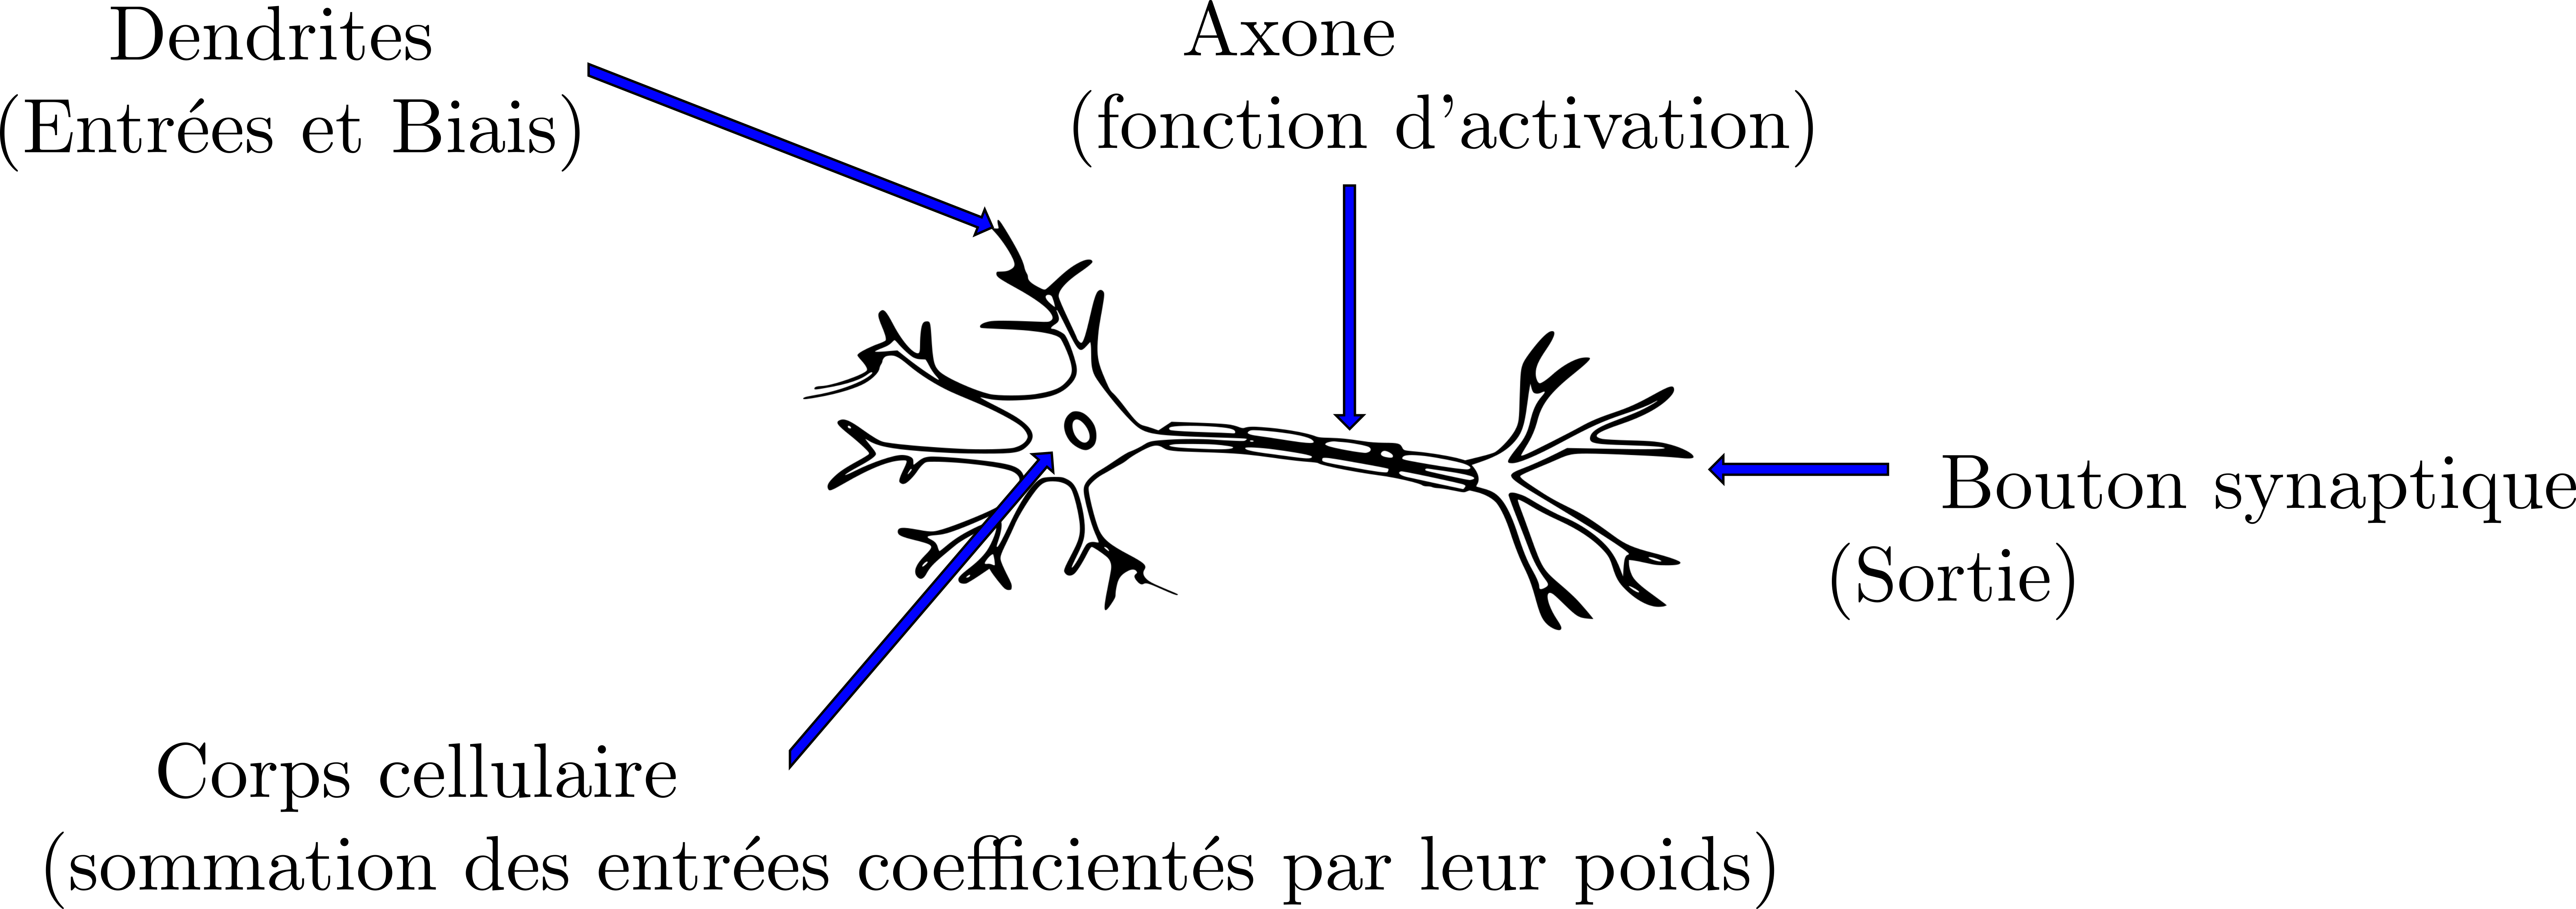
\includegraphics[height=75px]{2-Neurone.png}
		\caption{Schéma d'un neurone humain}
	\end{figure}
\end{frame}

\begin{frame}{I - Le perceptron}
	\begin{figure}
		\centering
		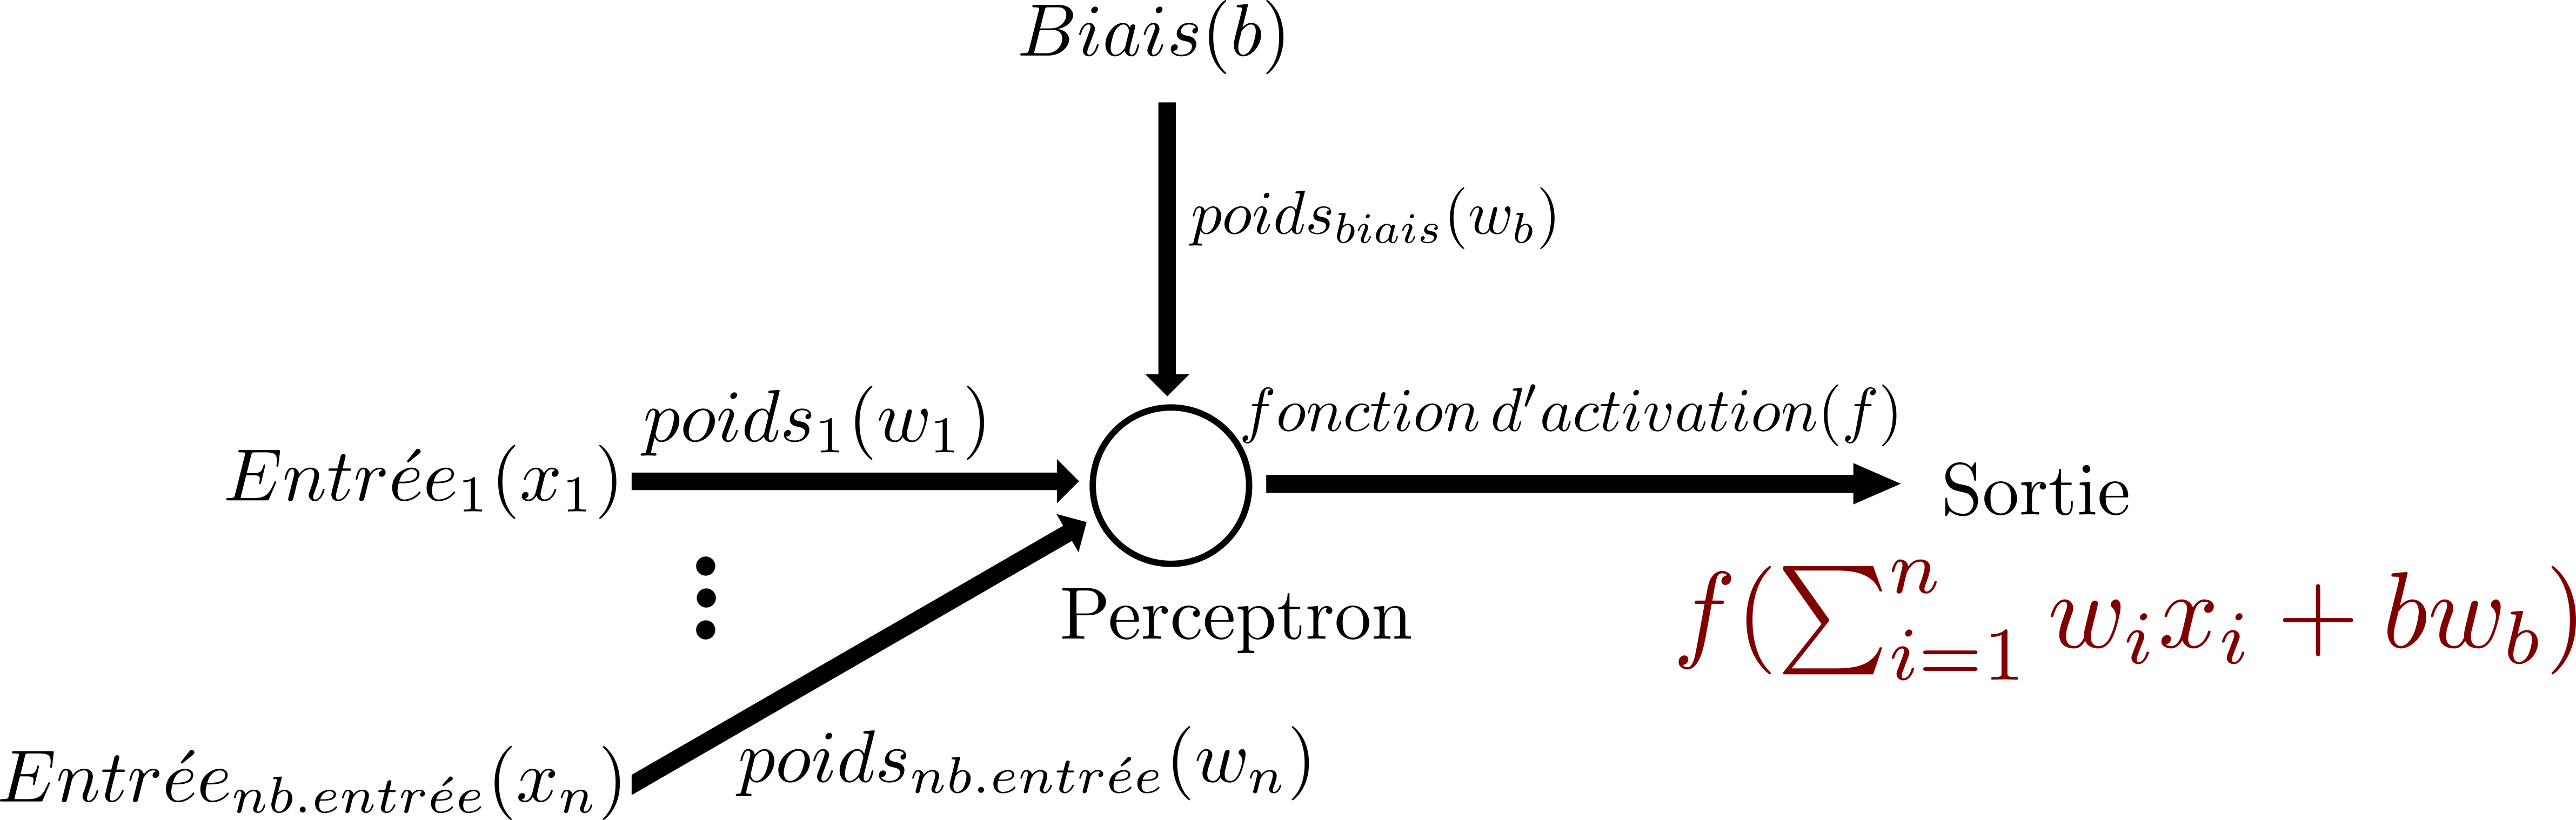
\includegraphics[height=120px]{1-Perceptron.png}
		\caption{Schéma d'un perceptron}
	\end{figure}
\end{frame}



\begin{frame}{I - Représentation informatique}
	\begin{figure}
		\centering
		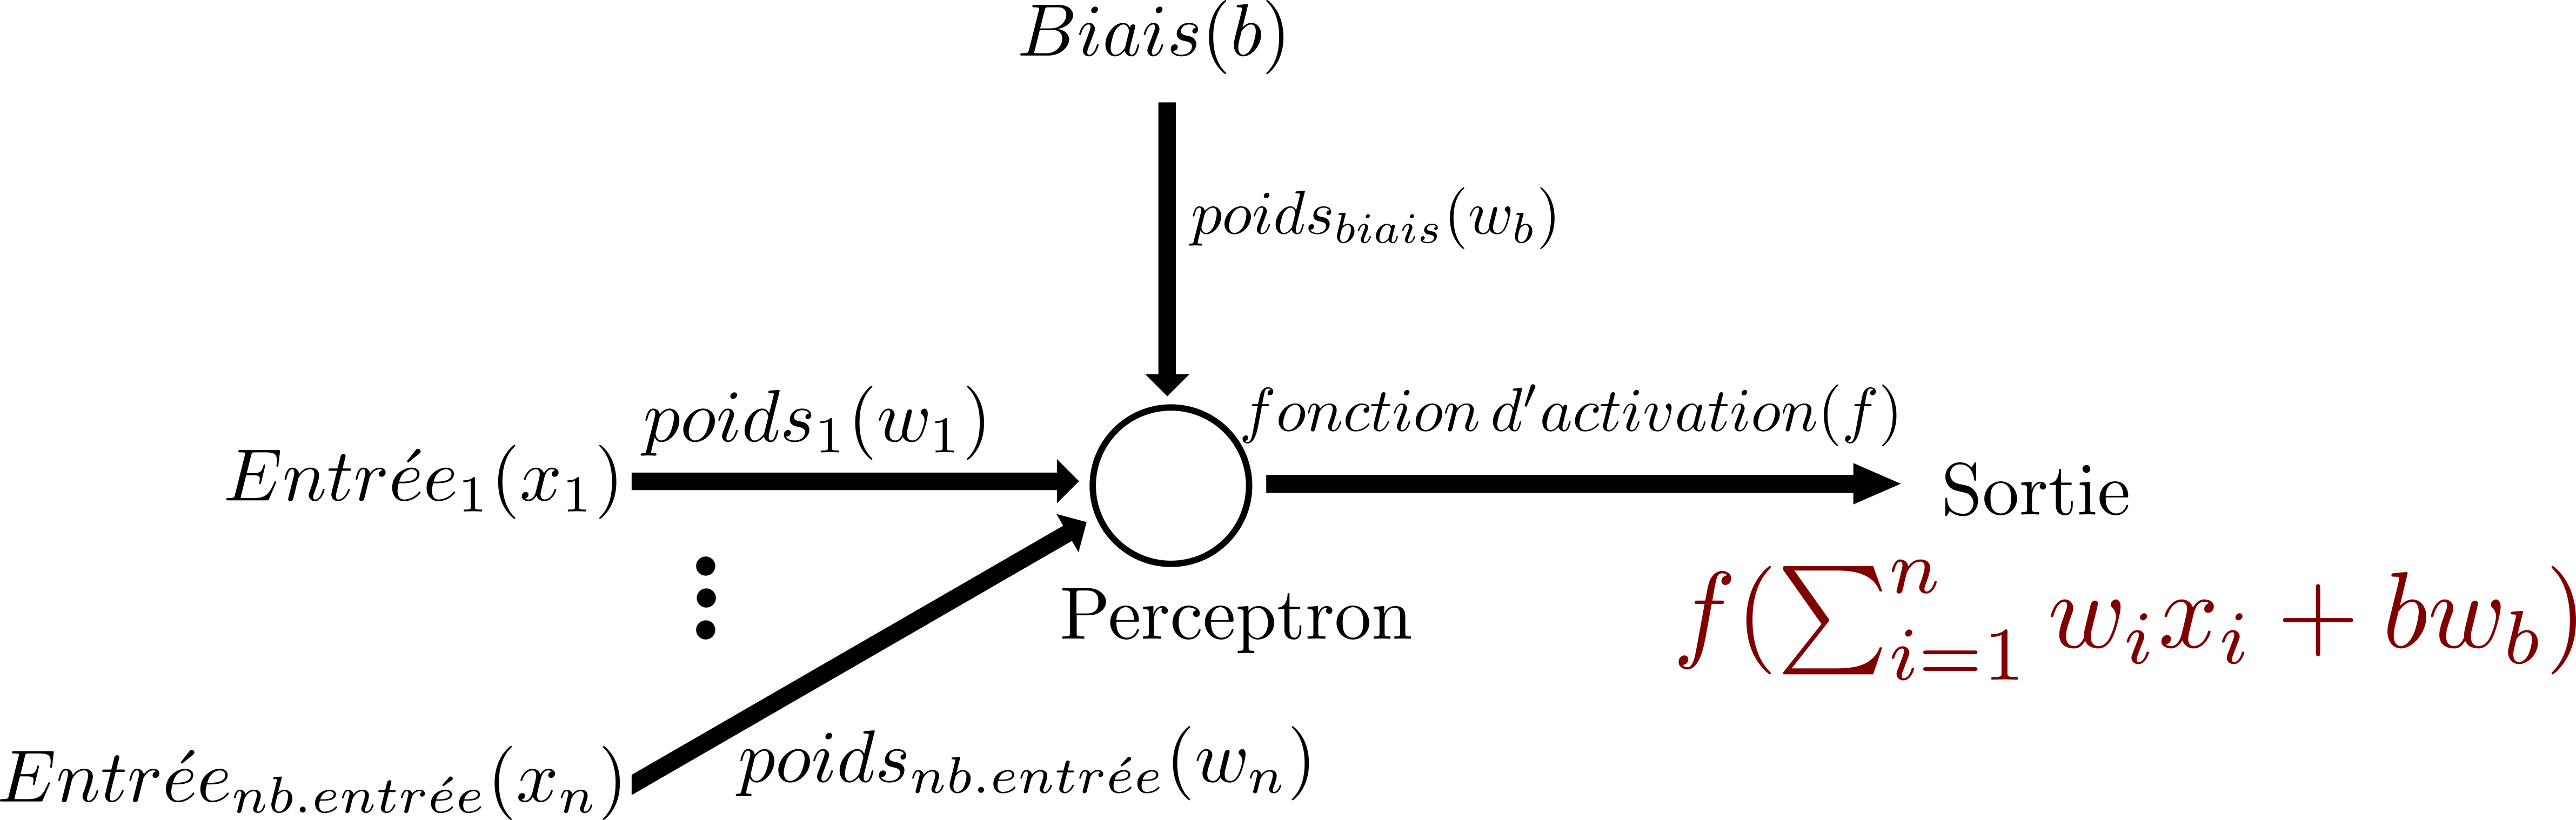
\includegraphics[height=75px]{1-Perceptron.png}
		\caption{Schéma d'un perceptron}
	\end{figure}
	\begin{multicols}{2}
		$
			f
			\left(
			\begin{pmatrix}
					x_1 & \ldots & x_n & b
				\end{pmatrix}
			\times
			\begin{pmatrix}
					w_1    \\
					\vdots \\
					w_n    \\
					w_b
				\end{pmatrix}
			\right)
		$ \\
		La complexité de $calcul$ est en $O(n)$
		\columnbreak
		\lstinputlisting[language=Python]{code.py}
	\end{multicols}
\end{frame}